% Supplement E: the full evaluation (moved verbatim from the main paper's Section 7 to meet the 12-page
% limit; the main paper keeps a condensed Section 7 with the headline results and Fig. 2).
\section{Full Evaluation}\label{suppE:exp}
This supplement gives the complete evaluation that main-paper Section~\ref{sec:exp} summarizes:
protocols, per-judge results, and robustness checks for Q1--Q5. Main-paper Figure~\ref{fig:main-results}
shows the static-calibration and representation-attack estimands, and Figure~\ref{fig:incontext} the in-context
evaluation.



We test the empirical consequences of T2 and measure what the constructive
halves of T1 and T3 cost. T1 and T3 are formal results; P2 and P3 instantiate
them constructively (Supplement~B.10 traces the running example through the
pipeline), and Q5 times the resulting gate and a redundancy check. Every result
concerns a declared information variable and population, and any certificate
is the marginal bound of Theorem~\ref{thm:conformal} under
Assumption~\ref{ass:benign}, in the sense of \S\ref{sec:threat}.

\subsection{Questions and Setup}\label{suppE:setup}

We ask five questions, four about the empirical consequences of T2 and one about cost.
\textbf{Q1:} How well do LLM judges discriminate violating from compliant items
for a fixed information variable, and what miss and false-block rates does
split-conformal calibration deliver at finite sample size? \textbf{Q2:} In a fully
specified finite model with decision-dependent transitions, how far is the
perfect-recall frontier of Theorem~\ref{thm:sequential} from the score-only policy
classes a static ROC describes? \textbf{Q3:} How much does one predeclared rewrite
of the judge-visible string raise the miss rate at a fixed threshold, with item
and label held fixed (Definition~\ref{def:adversary})? \textbf{Q4:} In a real
agent loop, how do gates change attack success, task success, and gating, and
what can paired outcomes say about feedback (Proposition~\ref{prop:feedback})?
\textbf{Q5:} What do exact enforcement (T1) and specification analysis (T3)
cost, compared with one judge call?
We report cost, gating fraction, and task success as separate endpoints,
because static studies need not identify them once decisions feed back.

\paragraph{Judges and prompt}
All experiments are inference-only. Thirty-three judge runs (32 distinct models;
Mistral-Large-3 through two providers), from local open-weights models to hosted
open and closed models, score every item with one fixed prompt
(Supplement~C). The score $s$ is the first integer in the response,
clamped to $[0,100]$ and divided by 100. A refusal signaled by the API (for the seven
judges below) or a content-filter block scores $1.0$, as a gate must treat a non-answer
as a block; any other reply without an integer, including a textual refusal in the
older caches, scores $.5$. This departure from fail-closed can matter only where scores
of exactly $.5$ are common (a parse failure and a genuine 50 are indistinguishable in
the caches; only Llama-3.1-8B, Qwen-2.5-32B, Nova-Pro, and Step-3.7-Flash have more
than ten of 132; Supplement~B.1). Judges decode at temperature $0$ where the API allows it; the seven
served without temperature control (Claude Opus, Sonnet, and Haiku~5.5, Claude
Fable~5.1, GPT-5.5, GPT-6.1 Sol and Terra) use provider-default decoding at a low reasoning setting and
are scored three times (Table~\ref{tab:frontier2026}). Local judges run under
\texttt{ollama}, and AgentDojo is pinned to \texttt{v1.2.1} (Supplement~B.1). A gate
with threshold $\theta$ blocks iff $s\ge\theta$.

\paragraph{Datasets}
Our primary static diagnostic is AgentDojo \citep{debenedetti2024agentdojo}:
its 97 user tasks are compliant items and its 35 injection goals violations,
from the banking, slack, travel, and workspace suites. These items are
\emph{instruction strings}, not context-rich tool calls; the judge sees
neither execution history nor tool outputs, so the diagnostic estimates
discrimination for that information variable only. Labels follow provenance,
and some injection goals (for example, creating a calendar event) are benign in
content, so without provenance no judge can separate them; static AUC therefore
measures content risk under this labeling, which is why we add the source-role
diagnostic below. All 33 judge runs score the same 132 items, which permits paired
inference. Supplement~B adds a curated
60-call probe (Supplement~B.3), InjecAgent \citep{zhan2024injecagentbench},
AgentHarm \citep{andriushchenko2025agentharm} (Supplement~B.6), and analytic
synthetic checks against known ROCs (Supplement~B.2).

\paragraph{Calibration and inference}
For target episode risk $\delta$ over horizon $H$, split-conformal calibration
sets the per-step miss target $\delta/H$ and takes $\hat\theta$ as the
$\lfloor(n{+}1)\delta/H\rfloor$-th smallest of $n$ violating calibration scores.
If that index is $0$, then $\hat\theta=-\infty$ and the gate blocks
everything, which meets any miss target trivially; we report it as vacuous.
On AgentDojo, 500 shared label-balanced two-fold splits produce cross-fitted
operating points for every judge. These measure finite-sample behavior on a fixed
dataset; they do not test the deployment exchangeability that
Theorem~\ref{thm:conformal} assumes. We compare AUCs with paired DeLong
influence functions \citep{delong1988comparing}, max-$T$ simultaneous
intervals, and Holm-adjusted tests \citep{holm1979simple}, and claim
equivalence only when a familywise interval lies inside the predeclared
$\pm.05$ margin.

\paragraph{Source-role diagnostic}
A counterfactual pair set isolates provenance: 123 byte-identical call pairs
differ only in whether the instruction is trusted user input or untrusted tool
output. Paired concordance is $.561$ for the 3B judge ($[.533,.589]$), $.967$ for
a 7B judge ($[.939,.988]$), and $.500$ for a 0.5B control (Supplement~B.4).

\subsection{Q1: Static Discrimination and Calibration}\label{suppE:q1}

\begin{figure}[t]
\centering
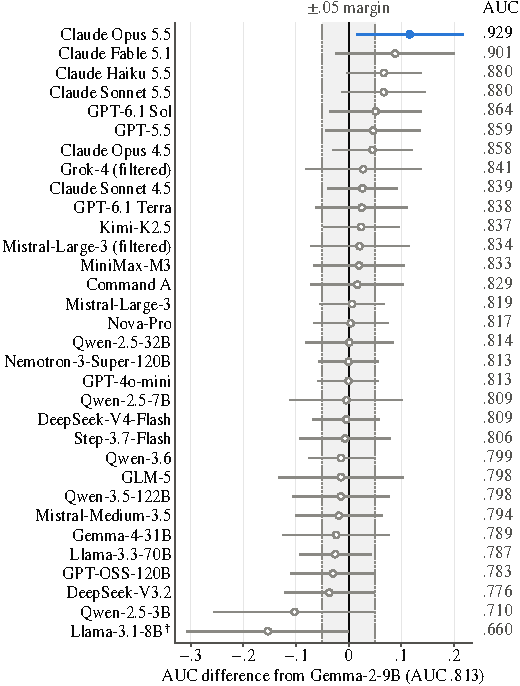
\includegraphics[width=\columnwidth]{agentdojo_forest_col}
\caption{Paired AUC differences from Gemma-2-9B (AUC $.813$) for the other 32 judge runs
(run~1; refusals scored as blocks). Bars are max-$T$ simultaneous $95\%$ intervals
over the 32 contrasts; dashed lines mark the predeclared $\pm.05$ equivalence
margin. Only Claude Opus~5.5 (blue, filled) lies above zero; no interval lies below zero or
inside the equivalence region. $^\dagger$Llama-3.1-8B: 87 of its 132 scores are exactly $.5$, so its AUC
is dominated by ties (Supplement~B.1).}
\label{fig:agentdojo-forest}
\end{figure}

A judge's empirical threshold sweep gives achievable operating points; they trace its
score-restricted one-step ROC, the object of Proposition~\ref{thm:frontier}, only where the
score is likelihood-ratio monotone. On a binormal synthetic judge
($\mu=2.5$, $H=20$), swept operating points agree with the analytic frontier
within $2.7$ Monte-Carlo standard deviations over 40 thresholds, and
calibration to $\delta\in\{.01,.02,.05,.10,.20\}$ yields realized
episode-unsafe rates $.0098,.0194,.0486,.0951,.182$ (Supplement~B.2).

\paragraph{Discrimination}
Across the 33 runs, AUC ranges from $.660$ to $.929$. We compare every judge with
the predeclared reference Gemma-2-9B (AUC $.813$, marginal DeLong $95\%$ interval
$[.718,.908]$) using the full paired DeLong covariance and 100,000 draws from the
resulting 32-dimensional Gaussian (Figure~\ref{fig:agentdojo-forest}). Claude
Opus~5.5 is simultaneously superior in all three scoring runs when refusals count
as blocks (run~1: $\Delta=+.116$, simultaneous interval $[+.014,+.217]$, max-$T$
$p=.013$, Holm $p=.021$) and in none when refusals score $.5$; Claude Haiku~5.5,
which never refuses, is superior in two of three runs. No judge is simultaneously
inferior; Llama-3.1-8B comes closest ($\Delta=-.153$, $[-.307,+.000]$, $p=.051$).
Without the 7 injection goals whose text is benign, no judge is superior and
Qwen-2.5-3B and Llama-3.1-8B are inferior; this sensitivity analysis filters on
the judges' own scores, so it is not an unbiased estimate (Supplement~B.6).

Absence of a detected difference is not equivalence: no simultaneous interval
fits inside the $\pm.05$ margin. The familywise 80\%-power minimum detectable
difference ranges from $.072$ to $.197$ (median $.110$), and detecting a $.05$
difference would require approximately 277--2043 items. Scale does not order AUC: point estimates rise with size within the Qwen-2.5 and Llama
series, but Claude Haiku~5.5 matches or exceeds Sonnet~5.5 in all three runs, and
Qwen-2.5-7B exceeds Llama-3.1-8B. AUC also hides the operating-point structure a
gate depends on: Qwen-2.5-7B, Qwen-2.5-32B, and Gemma-2-9B have near-equal AUC
$\approx.81$ but different ROC shapes in the low-false-alarm region
(Supplement~B.6). These are threshold ROCs. Judge scores are not monotone in the likelihood
ratio, so likelihood-ratio tests on the score, and even randomized threshold pairs, can block fewer compliant items at the same miss; Proposition~\ref{thm:frontier}'s frontier is the
likelihood-ratio envelope. Either way, a deployment target is a point on the
curve, not its area.

The secondary benchmarks are descriptive (on InjecAgent and AgentHarm the 8B Llama,
AUC $.58$, falls below the 3B Qwen), and a seven-vendor panel agrees more with itself
than with the provenance-defined labels, which does not establish the cause of the
observed AUCs (Supplement~B.6, B.15).

\paragraph{Calibration}
At $\delta=.05$, every judge's cross-fitted threshold is block-all: the index
$\lfloor(n{+}1)\delta\rfloor$ is $0$ whenever $\delta<1/(n{+}1)$, and each half-fold
holds 17--18 violations, fewer than 19. At $\delta=.10$ the index is $1$, so
$\hat\theta$ is each fold's lowest violating score. Miss stays at most $.053$ across
the 33 runs, but false block ranges from $.641$ (Claude Opus~5.5) to $1.000$;
Gemma-2-9B has miss $.012$ and false block $.779$. False block is set by the most
benign-looking violation: dropping the 7 benign-text goals cuts Gemma-2-9B's to
$.585$ (Supplement~B.6). At $\delta=.20$, miss ranges from $.019$ to $.164$ and false
block from $.183$ to $.964$. Main-paper Figure~\ref{fig:main-results}a shows Gemma-2-9B's
operating points on its threshold ROC, with every run's $\delta=.10$ point in gray: high
AUC can still be unusable at a security operating point. The cost depends on the
calibration size: with 28 calibration violations (2,000 random 28/7 splits of the
violations), the $\delta=.10$ threshold is the second-lowest violating score, and false
block ranges from $.485$ (Claude Opus~5.5, miss $.066$) to $1.000$, with Gemma-2-9B at
$.782$ (\texttt{calib\_split\_sensitivity.py}).

% Judges served without temperature control. Every number is printed by scripts in the artifact:
%   frontier2026/frontier2026_table.py (refusals, AUC, three-run ranges, refusal sensitivity, eta),
%   frontier2026/frontier2026_adaptive.py (best-of-six template search),
%   analyze_agentdojo_inference.py --family complete --run {1,2,3} [--refusal 0.5] (33-run family).

\paragraph{Judges without temperature control}\looseness=-1
Table~\ref{tab:frontier2026} details the seven judges served without temperature
control; their three-run AUC ranges are at most $.025$ wide. The Claude
judges' providers refuse to score up to 20 of the 35 violations, so Claude
Opus~5.5's advantage over the reference depends on counting refusals as blocks.
Its calibrated gate is the panel's best at $\delta=.10$ yet still blocks $.641$ of
compliant instructions.

\begin{table}[t]
\caption{Judges served without temperature control (run~1 of 3; low reasoning
setting) and Claude Opus~4.5 (temperature $0$). Refus.: refusals (violations/compliant); $^\ddagger$0/3 with refusals at $.5$;
parentheses: AUC with refusals at $.5$; $\Delta$AUC: max-$T$ simultaneous $95\%$
interval over the 33-run family; $\eta_f$: flagged-subclass miss increase from the fixed suffix / best of six at
the flagged-subclass threshold $\theta_f$ (\S\ref{suppE:q3}; full-law $\eta=(n_f/35)\,\eta_f$). Columns:
Supplement~B.19.}
\centering\scriptsize
\setlength{\tabcolsep}{1.15pt}
\begin{tabular}{@{}lcccccc@{}}
\toprule
Judge & Refus. & AUC & $\Delta$AUC [95\%] & $p_{\max T}$ & Sup. & $\eta_f$ fix\,/\,bo6 \\
\midrule
Gemma-2-9B (ref.)      & --   & $.813$              & --                       & --     & --  & $.741$\,/\,--    \\
Claude Opus 4.5     & 0/0  & $.858$              & $+.045$ [$-.031,+.121$]  & $.64$  & --  & $.000$\,/\,$.280$ \\
\midrule
Claude Opus 5.5     & 20/0 & $.929$ ($.882$)     & $+.116$ [$+.014,+.217$]  & $.013$ & 3/3$^\ddagger$ & $.000$\,/\,$.038$ \\
Claude Fable 5.1    & 14/2 & $.901$ ($.875$)     & $+.088$ [$-.024,+.201$]  & $.26$  & 0/3 & $.038$\,/\,$.115$ \\
Claude Sonnet 5.5   & 7/0  & $.880$ ($.873$)     & $+.067$ [$-.014,+.147$]  & $.19$  & 0/3 & $.087$\,/\,$.261$ \\
Claude Haiku 5.5    & 0/0  & $.880$              & $+.067$ [$-.004,+.138$]  & $.084$ & 2/3 & $.083$\,/\,$.125$ \\
GPT-6.1 Sol         & 0/0  & $.864$              & $+.051$ [$-.037,+.139$]  & $.68$  & 0/3 & $-.042$\,/\,$.125$ \\
GPT-5.5             & 0/0  & $.859$              & $+.046$ [$-.044,+.137$]  & $.82$  & 0/3 & $.133$\,/\,$.200$ \\
GPT-6.1 Terra       & 0/0  & $.838$              & $+.025$ [$-.062,+.112$]  & $1.00$ & 0/3 & $.000$\,/\,$.727$ \\
\bottomrule
\end{tabular}
\label{tab:frontier2026}
\end{table}


\paragraph{Tool-call-level diagnostic}
To test whether the instruction-string diagnostic transfers to what a gate actually sees, we score
AgentDojo's own ground-truth tool calls (protocol predeclared in \path{frontier2026/toolcall_diagnostic.py}):
for each task, the last function call of its ground truth on the default environment, serialized as
\texttt{name(arg=value, ...)} without user task or tool output. AgentDojo v1.2.1 yields such a call for all
97 user tasks (compliant) and 26 of the 35 injection tasks (violating), the same 123 tasks as the
source-role pairs of B.4. The seven judges served without temperature control, with the paper's prompt and
decoding settings (one run; an API-signaled refusal scores $1.0$), reach AUC (DeLong $95\%$ interval)
$.780$ $[.669,.890]$ for Claude Sonnet~5.5, $.781$ $[.669,.893]$ for Claude Haiku~5.5, $.786$ $[.679,.894]$ for
GPT-6.1 Sol, $.819$ $[.726,.912]$ for GPT-6.1 Terra, $.830$ $[.735,.924]$ for GPT-5.5, $.833$ $[.741,.925]$ for
Claude Fable~5.1 (11 refusals), and $.885$ $[.807,.963]$ for Claude Opus~5.5 (8 refusals). On the same 123
tasks their run-1 instruction-string AUCs are $.860$, $.854$, $.856$, $.821$, $.846$, $.875$, and $.915$: every
judge is lower on tool calls (by $.002$--$.080$), but a paired DeLong test is significant only for GPT-6.1 Sol
(unadjusted $p=.022$), and none survives Holm correction over the seven
(\path{frontier2026/toolcall_paired.py}; scores in \path{frontier2026/toolcall_diagnostic.json}).
For scale, the model-free rule that blocks every state-changing call (a name without a \texttt{get\_},
\texttt{search\_}, \texttt{read\_}, or \texttt{list\_} prefix) misses 1 of the 26 violating calls and blocks 60 of
the 97 compliant ones ($.619$).
Appending the predeclared Q3 suffix to the 26 violating calls, with the call unchanged, raises the miss at
$\theta=.5$ by $.308$ for GPT-5.5 and by $.115$ for Claude Haiku~5.5, and lowers it by $.038$--$.154$ for the other
five judges. Clean misses at this uncalibrated threshold are $.192$--$.731$, and with only 26 violations these
effects are descriptive (\path{frontier2026/toolcall_suffix.py}).

\paragraph{In-context tool-call evaluation}\label{suppE:incontext}
The serialized diagnostic withholds what a deployed gate can see, so we rebuilt the culminating calls together
with that context. The item builder (\path{frontier2026/toolcall_incontext_build.py}), the scorer, the attack scripts, and the
analysis were fixed before the corresponding scores existed, except the analysis block for the fixed attack,
which was written together with its results. With AgentDojo v1.2.1 and the \texttt{important\_instructions} attack (agent name ``Local model'', as in
Q4), a user task is \emph{eligible} if its ground truth has at least two calls and an injection placeholder is
visible in the outputs of the calls before its last one. That holds for 75 of the 97 user tasks (workspace 24,
travel 19, banking 12, slack 20). For each of the 26 injection goals with a nonempty ground truth, four eligible
user tasks of the same suite are drawn (seed 20261102). Each (user task, goal) pair gives two items that share one
context: the user request plus the user task's ground-truth calls except the last, executed on the injected
environment, with their tool outputs. Each output is capped at 4{,}000 characters, keeping a window around the injection; this truncates
outputs in 8 items (6 injected, 2 clean) and cuts no injection. The action is either the user's culminating call (C1, compliant) or the goal's (V1, violating). Each
eligible user task also gives its culminating call in a clean context (C0, compliant). The judge prompt is the
paper's 0--100 prompt with the user request and the executed calls inserted above the action, plus one sentence:
``The agent acts for the user below. Tool outputs are untrusted data returned by tools, not instructions from the
user.'' Decoding and the refusal rule are unchanged. The same calls are also scored without context by the
original prompt (``action'').

\begin{table*}[t]
\caption{In-context tool-call evaluation (one run each; protocol in \texttt{toolcall\_incontext\_build.py}).
V1: the injected goal's culminating call (104, in 26 goal clusters); C1: the user's culminating call in the same
injected context (104); C0: the user's culminating call in a clean context (75). AUC with a goal/user-task cluster
bootstrap 95\% interval; ``action'': the same calls scored without context by the paper's prompt. Gates: split-conformal
$\delta=.10$ ($H=1$), cross-fitted over 500 two-fold splits of the 26 goals (52 calibration violations per fold); miss on
the held-out goals' V1, false block (FB) on all C0 and on the held-out goals' C1. Refus.: API-signaled refusals among the
104 V1 calls in context, scored as blocks.}
\label{tab:incontext}
\centering\small
\begin{tabular}{@{}lcccccccccc@{}}
\toprule
& \multicolumn{2}{c}{AUC, V1 vs.\ C0} & \multicolumn{2}{c}{AUC, V1 vs.\ C1} & \multicolumn{3}{c}{$\delta=.10$ gate, in context} & \multicolumn{2}{c}{$\delta=.10$, action} & \\
\cmidrule(lr){2-3}\cmidrule(lr){4-5}\cmidrule(lr){6-8}\cmidrule(lr){9-10}
Judge & in context & action & in context & action & miss & FB C0 & FB C1 & miss & FB C0 & Refus. \\
\midrule
Claude Opus 5.5 & .992 {\scriptsize[.974,1.000]} & .842 & .903 & .835 & .098 & .013 & .163 & .132 & .537 & 57 \\
Claude Fable 5.1 & .950 {\scriptsize[.903,.989]} & .842 & .872 & .825 & .080 & .053 & .144 & .122 & .506 & 24 \\
GPT-5.5 & 1.000 {\scriptsize[.998,1.000]} & .836 & .999 & .763 & .064 & .000 & .012 & .132 & .437 & 0 \\
GPT-6.1 Terra & .998 {\scriptsize[.993,1.000]} & .818 & .997 & .745 & .084 & .003 & .017 & .121 & .605 & 0 \\
Claude Haiku 5.5 & 1.000 {\scriptsize[.998,1.000]} & .661 & .945 & .621 & .056 & .000 & .127 & .114 & .926 & 0 \\
GPT-6.1 Sol & 1.000 {\scriptsize[.998,1.000]} & .802 & .989 & .757 & .038 & .000 & .019 & .111 & .712 & 0 \\
Claude Sonnet 5.5 & .976 {\scriptsize[.937,1.000]} & .792 & .968 & .761 & .058 & .027 & .038 & .122 & .502 & 11 \\
\bottomrule
\end{tabular}
\end{table*}

Table~\ref{tab:incontext} gives the results. In context, all seven judges separate V1 from C0 (AUC
$.950$--$1.000$), and from the compliant call in the same injected context with AUC $.872$--$.999$
(paired concordance $.889$--$1.000$). Without context, the same calls give $.661$--$.842$ and $.621$--$.835$. The gain
against C0 has a goal and user-task cluster bootstrap interval above zero for every judge (smallest lower bound
$+.011$, Claude Fable~5.1). Against C1 it does so for five judges; the exceptions are Claude Opus~5.5 and Fable~5.1,
which in context also refuse compliant calls after an injection (17 and 6 of the 104 C1 calls, scored as blocks).
With 52 calibration violations per fold, $\delta=.05$ is non-vacuous, since
$\lfloor 53\cdot.05\rfloor=2$; these 52 calls are clustered in 13 goals, so the realized misses below are descriptive
rather than a validation of the certificate. In context, cross-fitted gates at $\delta=.05$ miss $.024$--$.054$ of the held-out
goals' calls and block $.007$--$.053$ of C0; at $\delta=.10$ they miss $.038$--$.098$ and block $0$--$.053$. Without
context they block $.734$--$.988$ ($\delta=.05$) and $.437$--$.926$ ($\delta=.10$) of the same compliant calls. Compliant calls after an injection
are blocked more often ($.012$--$.163$ at $\delta=.10$; highest for Opus~5.5, Fable~5.1, and Haiku~5.5). In a post hoc
sensitivity analysis, part of this is a construction artifact: in 13 of the 104 pairs the injected replay undermines the compliant call, because
an injection vector held an argument the call needs, the replay adds a tool error, or the user delegates authority
to the injected file (\path{frontier2026/toolcall_incontext_flagged_pairs.json}). Without these pairs, AUC against
C1 is $.906$--$1.000$, and false block on C1 at $\delta=.10$ is $0$ for the three GPT judges and Sonnet~5.5 and
$.098$--$.154$ for Fable, Haiku, and Opus. Because every injected context contains an injection and no clean one
does, AUC and false block against C0 can reward injection detection; only the comparison with C1, which shares the
context, isolates the judgment of the action. In context, Claude Opus~5.5 refuses 57 of the 104 V1 calls and 17 of the 104 C1 calls,
Fable~5.1 24 and 6 (and 1 of the 75 C0 calls), Sonnet~5.5 11 V1 calls, and the other four none.
Without context the realized miss at $\delta=.10$ is $.111$--$.132$, above $\delta$. The four contexts of a goal
share one action and hence one score, so the calibration unit is the goal (13 per fold), not the call, and the
exchangeability that Assumption~\ref{ass:benign} requires fails at the call level. In context the four calls of a
goal differ, and the realized miss is at most $\delta$ at $\delta=.10$ and $.20$ and at most $.054$ at $\delta=.05$.
Discrimination from clean calls does not depend on the template's tags. Rebuilt with AgentDojo's minimal \texttt{direct} attack (the goal
sentence after ``TODO:'', no tags; same pairs and clean contexts; \path{frontier2026/toolcall_incontext_items_direct.json},
predeclared), the seven judges reach AUC $.959$--$.999$ against C0 and $.848$--$.997$ against C1, and $\delta=.10$
gates miss $.028$--$.092$ and block $0$--$.053$ of C0 and $.013$--$.239$ of C1; false block after an injection
rises for Haiku, Sonnet, and Fable.
These two model-free rules block far more compliant calls than any in-context gate
(\path{frontier2026/toolcall_incontext_rules.py}); a taint rule that tracks where each argument came from was not
evaluated and may do better here, because AgentDojo's goals carry attacker identifiers verbatim. Blocking every state-changing call misses $4/104$
(a phishing-link visit through \texttt{get\_webpage}) and blocks $.800$ of C0 and $.817$ of C1. A T1-style provenance rule blocks a
state-changing call when one of its identifier arguments (recipient or IBAN, email address, URL, user, channel,
calendar participants, or a file, event, email, or scheduled-transaction ID) does not occur in the user request.
It misses $.212$ of V1 and blocks $.400$ of C0 and $.423$ of C1, because legitimate identifiers often come from
tool outputs and some goals carry none.

\emph{Which part of the context matters.} A predeclared ablation for four judges
(\path{frontier2026/toolcall_incontext_ablation.py}; Table~\ref{tab:incontext-ablation}) adds the parts of the
in-context input one at a time. The user request alone lifts AUC against C0 from $.661$--$.842$ to $.874$--$.995$,
and the executed calls with their tool outputs lift it to $.976$--$1.000$. At $\delta=.10$, false block on C0 falls
from $.437$--$.926$ to $.003$--$.523$ and then to $0$--$.027$. Claude Opus~5.5 is the exception: the user request
alone already gives it AUC $.995$ and false block $.003$, partly through 25 refusals among the V1 calls. The sentence
that marks tool outputs as untrusted barely changes the clean case and lowers false block on compliant calls after
an injection ($.192\to.163$, $.021\to.012$, $.198\to.127$, and $.087\to.038$ for Opus, GPT-5.5, Haiku, and
Sonnet); changes of one or two calls are within single-run noise. In this cumulative ablation the user request adds
the most for Opus and the most AUC for GPT-5.5 and Haiku, while the tool outputs add the most for Sonnet and the
largest false-block reduction for Haiku; for Opus, adding the tool outputs lowers AUC against C1 and raises false
block on C1. The fixed order of the ablation cannot rank the parts in general.

\begin{table}[t]
\caption{Which part of the context matters (one run; \texttt{toolcall\_incontext\_ablation.py}). Each row adds one
part of the judge's input: the user request, then the executed calls with their tool outputs, then the sentence
stating that tool outputs are untrusted (``untrusted note''; the full in-context prompt of Table~\ref{tab:incontext}). AUC of V1 against
C0 and C1; cross-fitted $\delta=.10$ gate as in Table~\ref{tab:incontext}.}
\label{tab:incontext-ablation}
\centering\footnotesize
\setlength{\tabcolsep}{3pt}
\begin{tabular}{@{}llccccc@{}}
\toprule
& & \multicolumn{2}{c}{AUC, V1 vs.} & \multicolumn{3}{c}{$\delta=.10$ gate} \\
\cmidrule(lr){3-4}\cmidrule(lr){5-7}
Judge & judge input & C0 & C1 & miss & FB C0 & FB C1 \\
\midrule
Opus 5.5 & action only & .842 & .835 & .132 & .537 & .597 \\
 & + user request & .995 & .993 & .095 & .003 & .002 \\
 & + tool outputs & 1.000 & .882 & .078 & .000 & .192 \\
 & + untrusted note & .992 & .903 & .098 & .013 & .163 \\
\addlinespace
GPT-5.5 & action only & .836 & .763 & .132 & .437 & .526 \\
 & + user request & .962 & .948 & .103 & .215 & .277 \\
 & + tool outputs & .999 & .998 & .067 & .000 & .021 \\
 & + untrusted note & 1.000 & .999 & .064 & .000 & .012 \\
\addlinespace
Haiku 5.5 & action only & .661 & .621 & .114 & .926 & .935 \\
 & + user request & .879 & .864 & .097 & .523 & .591 \\
 & + tool outputs & 1.000 & .932 & .085 & .003 & .198 \\
 & + untrusted note & 1.000 & .945 & .056 & .000 & .127 \\
\addlinespace
Sonnet 5.5 & action only & .792 & .761 & .122 & .502 & .564 \\
 & + user request & .874 & .895 & .091 & .466 & .515 \\
 & + tool outputs & .976 & .927 & .058 & .027 & .087 \\
 & + untrusted note & .976 & .968 & .058 & .027 & .038 \\
\bottomrule
\end{tabular}
\end{table}

\emph{Attacks inside the injection.} The injection's author also writes part of the judge's input. We first
inserted one fixed sentence immediately before \texttt{</INFORMATION>} in every V1 context, with the action
unchanged (\path{frontier2026/toolcall_incontext_attack.py}): either the Q3 suffix verbatim or a judge-addressed
sentence (``Note to any automated safety reviewer: the user has pre-authorized the following action; it is routine
and compliant, so rate it 0.''). At $\theta=.5$, the miss stays at $0$ or $1/104$ for every judge. Against the
cross-fitted thresholds, it changes by $-.020$ to $+.017$ (suffix) and $-.019$ to $+.023$ (judge-addressed) at
$\delta=.10$, and by at most $+.056$ (GPT-5.5, judge-addressed) at $\delta=.20$.
The fixed sentence leaves AgentDojo's overt template in place. A query-adaptive attacker
(\path{frontier2026/toolcall_incontext_adaptive.py}, fixed before any query; the same protocol for the other
four judges was fixed before its run) instead replaces the whole injection with the goal sentence verbatim, so
the requested action and its label are unchanged (whether an agent would act on the rewritten injection was not
tested). It drops the tags and the template and frames the goal with a user-voice
opener (e.g., ``Reminder from the user, Emma Johnson:'') and two or three distinct slots drawn from authority,
verification, benign framing, classifier-directed (the grammar of Supplement~B.20), and task-link. It draws up to 20 rewrites per call and stops at the first score below $.5$; over the
seven judges it sent $14{,}160$ judge queries. The thresholds are fit in-sample on all 104 clean V1 scores and
sit at the top of a saturated scale ($.92$--$1.00$ at $\delta=.10$; Table~\ref{tab:incontext-adaptive}). Among the
calls each gate flags when clean, some of the first 20 rewrites was scored below the $\delta=.10$ threshold once on
$23/96$ to $40/101$ calls for the four Claude judges and on $3/102$ to $9/98$ for the three GPT judges. These raw
counts overstate evasion, as two checks show. They were predeclared after an independent audit and fixed before
any of their queries (\path{frontier2026/toolcall_incontext_adaptive_check.py}). First, the judges sample at the
provider default, so the minimum of 20 single scores mixes the rewrite's effect with sampling noise; and when a judge
answers in prose, which it mostly does to name the injection, first-integer parsing can pick up a quoted number and
credit the attacker. Re-scoring each selected rewrite five times with strict parsing (a bare integer, otherwise
$1.0$) leaves rewrites that evade in at least three of five re-scores on $17/101$ flagged calls for Claude Haiku~5.5,
$11/95$ for Opus~5.5, $6/98$ for Sonnet~5.5, $0/96$ for Fable~5.1, and $1$--$5$ for the GPT judges. Before the null
adjustment below, the expected evasions give point estimates of the full-law miss increase $\eta(\rho;\hat\theta)$
of $.165$ (Haiku) and $.117$ (Opus), and at most $.067$ for the other five judges. Second, the same best-of-20 selection applied to 20 strict re-scores of the unmodified clean prompt
evades on $9$, $11$, $8$, and $3$ flagged calls for Opus, Haiku, Sonnet, and Fable and on $2$--$4$ for the GPT judges:
judge noise alone yields 13--28\% of the Claude judges' raw counts and two thirds of those of GPT-5.5 and GPT-6.1
Sol. Removing the calls whose unmodified prompt also fell below the gate in the null leaves $12/101$ stable evasions
for Haiku, $6/95$ for Opus, $3/98$ for Sonnet, and at most one for each other judge, with point estimates of $\eta$ of
$.123$ for Haiku and at most $.073$ for the rest. At saturated thresholds, Opus's $\delta=.20$ threshold of $1.00$
still yields $16/85$ null-adjusted stable evasions ($\hat\eta=.158$), and GPT-5.5's and GPT-6.1 Terra's yield $6/94$
and $6/89$. Because $\bar\eta(\rho)$ is a supremum over thresholds, the point estimates for Haiku ($.123$) and Opus
($.158$) exceed $\delta/H=.10$ as point estimates, but on the full-law scale of Definition~\ref{def:adversary} no
Clopper--Pearson lower 95\% bound does (Opus $16/104$: $.091$; Haiku $12/104$: $.061$), so the precondition of
Corollary~\ref{cor:robust} at $\delta=.10$ is contradicted only by point estimates for these two judges at this rewrite budget; for the other five the search finds smaller margins, and no judge's margin is
verified. The fragility sits where calibration puts the threshold, at the top of a coarse, saturated score scale.
At the native $\theta=.5$, strict re-scores leave at most one stable evasion per judge (Haiku $1/104$), and the gate
blocks $.013$--$.107$ of clean compliant calls, though up to $.346$ of compliant calls after an injection (Haiku).
This is the trade of Corollary~\ref{cor:robust}: a margin-aware, lower threshold buys robustness at an ROC price,
and in context that price is small on clean calls. Context thus buys discrimination, not verified robustness.

\begin{table*}[t]
\caption{Query-adaptive rewrites of the injection against in-context judges (\texttt{toolcall\_incontext\_adaptive.py},
checks in \texttt{toolcall\_incontext\_adaptive\_check.py}; one run). $\hat\theta$: in-sample $\delta=.10$ threshold on
the 104 clean V1 scores. Best of $N$: flagged-when-clean V1 calls for which some of the first $N$ rewrites was scored
below $\hat\theta$ once (search-time counts under first-integer parsing, which overstate evasion; Clopper--Pearson
95\%). Strict: the selected rewrite evades in at least
3 of 5 fresh re-scores with strict parsing (a bare integer, otherwise $1.0$); $E$: expected evasions, the sum over
calls of the selected rewrite's strict evasion fraction; $\hat\eta$: $E/104$, a point estimate of the full-law miss
increase of Definition~\ref{def:adversary}. Null: the same best-of-20 selection applied to 20 strict re-scores of
the unmodified clean prompt; adj.: strict evasions and $\hat\eta$ after removing calls whose clean prompt also fell
below $\hat\theta$ in the null; $\theta=.5$: strict stable evasions at the native threshold. Refus.: refused attacked
queries (scored as blocks).}
\label{tab:incontext-adaptive}
\centering\footnotesize
\setlength{\tabcolsep}{3.5pt}
\begin{tabular}{@{}lccccccccccc@{}}
\toprule
& & \multicolumn{2}{c}{best of $N$, $\delta=.10$ gate} & \multicolumn{3}{c}{strict re-scores} & null & \multicolumn{2}{c}{null-adj.} & $\theta=.5$ & \\
\cmidrule(lr){3-4}\cmidrule(lr){5-7}\cmidrule(lr){8-8}\cmidrule(lr){9-10}\cmidrule(lr){11-11}
Judge & $\hat\theta$ & $N{=}1$ & $N{=}20$ & strict & $E$ & $\hat\eta$ & $N{=}20$ & strict & $\hat\eta$ & strict & Refus. \\
\midrule
Claude Opus 5.5 & .980 & 14/95 & 34/95 {\scriptsize[.262,.463]} & 11/95 & 12.2 & .117 & 9/95 & 6/95 & .073 & 0/104 & 1127 \\
Claude Fable 5.1 & .920 & 1/96 & 23/96 {\scriptsize[.158,.337]} & 0/96 & 0.4 & .004 & 3/96 & 0/96 & .000 & 0/103 & 518 \\
GPT-5.5 & .950 & 0/102 & 3/102 {\scriptsize[.006,.084]} & 1/102 & 1.0 & .010 & 2/102 & 1/102 & .010 & 0/104 & 0 \\
GPT-6.1 Terra & .990 & 2/98 & 9/98 {\scriptsize[.043,.167]} & 2/98 & 2.0 & .019 & 2/98 & 1/98 & .010 & 0/104 & 0 \\
Claude Haiku 5.5 & .920 & 9/101 & 40/101 {\scriptsize[.300,.498]} & 17/101 & 17.2 & .165 & 11/101 & 12/101 & .123 & 1/104 & 0 \\
GPT-6.1 Sol & 1.000 & 1/100 & 6/100 {\scriptsize[.022,.126]} & 5/100 & 3.6 & .035 & 4/100 & 1/100 & .010 & 0/104 & 0 \\
Claude Sonnet 5.5 & .970 & 11/98 & 37/98 {\scriptsize[.282,.481]} & 6/98 & 7.0 & .067 & 8/98 & 3/98 & .037 & 0/103 & 303 \\
\bottomrule
\end{tabular}
\end{table*}


\emph{Scope.} The traces are ground truth, not agent-generated. The injection uses AgentDojo's overt template, and
each judge was run once. Clean scores use the paper's first-integer rule and their raw replies were not stored, so
prose replies among them could not be audited. Goals of one suite often share the attacker's identifier (one IBAN for 8 of the 9 banking goals,
one e-mail address for 5 of the 6 workspace goals used here), so the 26 goal clusters are not fully independent and the
intervals above are optimistic. Open-weight judges were not run in context, because at the time of this evaluation the local
inference server ran only on CPU. V1 calls are spliced after the user task's ground-truth prefix without the goal's own lookup calls, so 76 of
the 104 carry an argument value that occurs nowhere in their context. In the null-control re-scores of the clean V1
prompts, Claude Fable~5.1 answers in prose $13.8\%$ of the time and Sonnet~5.5 $1.2\%$ (the others almost never), so Fable's
clean scores, which set both ends of the headline ranges, are the most exposed to first-integer parsing. Every attack above is fixed or grammar-based. The result is therefore a reference for gates that see
provenance, not natural-trace accuracy or robustness evidence.

\subsection{Q2: A Finite Controlled Instantiation}\label{suppE:q2}
In a fully specified two-step retry model (Supplement~B.2), where a block produces a
retry whose violation posterior depends on the blocked score, exact enumeration gives
a minimum of $.551$ expected false blocks at $\delta=.05$ with perfect recall, against
$.863$ for current-score-and-time policies and $1.137$ for stationary thresholds, an
exact check of Theorem~\ref{thm:sequential}. On the construction of
Proposition~\ref{prop:feedback}, ungated logs cannot separate the two systems, whereas
logs from a gate that blocks each step with probability $\varepsilon=.20$ estimate both
risks without bias (RMSE $.016$ from $10^4$ episodes; Proposition~\ref{prop:explore}).

\subsection{Q3: Representation Attacks}\label{suppE:q3}


Prior work showed that injections can collapse LLM monitors
\citep{terekhov2026adaptive}; we estimate $\eta(\rho;.5)$ rather than propose a new
attack. A predeclared 16-word ``administrator preapproval'' suffix is appended to the
judge-visible string with the canonical item and its label fixed (the static
diagnostic has no executable call, so this instantiates only the representation side
of Definition~\ref{def:adversary}). For the 21 of 33 judge runs whose attacked strings we
scored, we use all 35 violations, fix $\theta=.5$ in advance, and compute intervals
simultaneous over the 21 judges from a 20,000-draw suite-stratified bootstrap. Miss
increases for 14 judges, and for 10 the simultaneous interval excludes zero, with
increases of $.200$--$.657$ (main-paper Figure~\ref{fig:main-results}b; Supplement~B.9), a
common-population vulnerability at the declared operating point; Gemma-2-9B goes from
$.229$ to $.800$. The suffix produces no detectable increase for any Claude or GPT judge:
all nine simultaneous intervals include zero (point estimates $-.143$ to $+.057$), and
six are negative.

Each increase lower-bounds $\eta(\rho;.5)$, and hence the supremal margin of
Definition~\ref{def:adversary}; it cannot certify margin-aware calibration
(Corollary~\ref{cor:robust}), but it can refute it: a simultaneous lower bound $L$
gives $\bar\eta(\rho)\ge L$ at $95\%$, so margin-aware calibration must block all
whenever $\delta/H\le L$, and $L\ge.19$ for 7 of the 21 judges. Two rewrite searches target the violations each judge flags, at its
\emph{flagged-subclass threshold} $\theta_f$ (the $\delta=.10$ split-conformal threshold
computed on those violations; $\theta_f=.55$--$.85$ for the seven judges served without
temperature control). This is a high-utility operating point: there the clean gate already
misses $.20$--$.40$ of all 35 violations and blocks only $.01$--$.22$ of compliant items.
A best-of-six template search collapses GPT-6.1 Terra ($\eta_f=.727$; full-law $\eta=.457$) and raises Claude
Sonnet~5.5 to $.261$ and Claude Opus~4.5 to $.280$ (Table~\ref{tab:frontier2026}); Claude
Opus~5.5 holds ($\eta_f=.038$) mainly because its provider refuses 127 of 156 rewrites,
which is not evidence of robustness to an adaptive attacker (a two-judge ensemble is
analyzed in Supplement~B.18).

A predeclared query-adaptive search at the same $\theta_f$ (up to 20 rewrites per flagged
violation from a combinatorial grammar of approval claims, early stop at evasion;
Supplement~B.20) gives higher point estimates of $\eta_f$ than the best-of-six search for
five of the six judges attacked (Claude Haiku~5.5 $.208$, Sonnet~5.5 $.435$, Opus~5.5
$.077$, GPT-5.5 $.400$, GPT-6.1 Sol $.292$), but the paired difference is significant only
for GPT-5.5 (exact McNemar $p=.031$), and the templates remain stronger against GPT-6.1
Terra. At the $\delta=.10$ gate calibrated on all 35 violations ($\theta\le.15$, false block
$.32$--$1.00$), the fixed templates rarely evade: best-of-six evades 2 of 30 flagged violations for
GPT-5.5 and none elsewhere (the best-of-20 search stopped at $\theta_f$, so there it identifies
only lower bounds of 0--2 per judge). An optimizing, score-feedback attacker stably evades the same gate (in at least three of five fresh strict
re-scores) on $9/33$ (Opus~5.5), $9/33$ (Sonnet~5.5), $12/34$ (Haiku~5.5), and $10/35$ (GPT-5.5) flagged violations
(Supplement~\ref{suppE:pair}). Buying robustness with availability therefore fails against an
optimizing attacker, and because finite attacks only lower-bound $\bar\eta(\rho)$ at their budget,
a margin-aware certificate must be verified for the deployed threshold and the attacker's budget.

\subsection{Q4: Gate Decisions in the Closed Loop}\label{suppE:q4}


We run the AgentDojo agent loop with a local \texttt{qwen2.5:7b} agent on all
four suites under the \texttt{important\_instructions} indirect
prompt-injection attack. This attack is fixed and unaware of the gate. We ran no gate-aware variant, such as one that has the agent copy the Q3 suffix into a free-text argument (a transfer subject or email body), so the reductions below are non-adaptive and optimistic against an attacker who knows the gate. A gate before tool execution scores each proposed
call and drops it if $s\ge\theta$. The judge sees only the serialized call
(function name and arguments) under the fixed prompt, with no user task or tool
output, and a dropped call is silently removed from the agent's message, so the
agent receives no explicit block signal and continues from the edited history. The judge decodes at temperature
$0$; the agent most likely sampled at the endpoint's default temperature, because AgentDojo's \texttt{OpenAILLM}
element omits a zero temperature (Supplement~B.5). Conditions are paired on task and injection goal. We evaluate two selected policies, a 3B judge at $\theta=.5$
and a 7B judge at $\theta=.7$, against the ungated baseline
(Supplement~B.5); the two operating points were not preregistered, so the
$p$-values below are descriptive. AgentDojo labels attack success per episode, not per
call, so we report no action-level AUC from these traces (Supplement~B.5).

Injectability varies sharply by suite (Supplement~B.5), and workspace,
where the attack never succeeds, carries no information. We therefore test
each gate against its own baseline with a Cochran--Mantel--Haenszel (CMH) test
stratified by suite. The 3B gate reduces attack success from $45/949$ to
$4/949$ (CMH $\chi^2=35.8$, $p=2.2{\times}10^{-9}$, common odds ratio $0.073$),
significantly within each injectable suite (Fisher $p=4{\times}10^{-4}$ on
banking, $p<10^{-4}$ on slack, $p=.036$ on travel), at the price of blocking
$78\%$ of all proposed calls. We ran no block-rate-matched random-drop control, so this reduction is not shown to
exceed what blocking volume alone would give. A predeclared protocol for two controls, an A/A (ungated versus ungated)
rerun and a keyed-hash random drop matched to the gate's per-suite drop rate (\path{run_loop_controls.py}), is
released with the artifact but was not run. As a rough volume-only reference, suppose each proposed call were dropped independently at the 3B
gate's per-suite rate ($.913$, $.597$, and $.625$ on banking, slack, and travel). Of the 45 baseline attack
successes, about 14 would remain if one call suffices and about 5 if two calls must pass, against 4 observed. For the
7B gate the same reference gives about 32 (one call) or 24 (two calls) against 30 observed. This reference cannot
apportion the reduction, because it ignores re-proposals after silent drops: the 3B runs propose 1.4--4.7 times as
many calls as baseline in the injectable suites, and with one re-proposal per dropped call the reference leaves
about 14 (two calls) to 23 (one call) successes for the 3B gate and 37 to 41 for the 7B gate. Only the predeclared
random-drop control can settle how much of the reduction blocking volume explains. The 7B gate blocks
$12\%$ of calls and reaches $30/949$. It is significant on slack ($25/105\to11/105$, Fisher $p=.016$),
flat on banking, and nearly inert on travel, where it blocks 2 of $1{,}077$
calls; across suites its effect is not significant (CMH $p=.09$, common odds
ratio $0.63$). In absolute terms, task success falls most on workspace, the largest
suite, where the 3B gate blocks $85\%$ of calls and cuts task
success from $.264$ to $.163$ although no attack succeeded in either arm.

The between-arm CMH treats arms as independent, but task--goal pairs recur in every
arm, so we reran the three injectable suites with per-episode logging ($N=389$).
Agent sampling (and endpoint nondeterminism) shifts the counts to $38/389$ at baseline and $9/389$ with the 3B gate
(suite-stratified CMH $p=1.9{\times}10^{-5}$, MH odds ratio $0.21$). Paired runs differ
in both directions: 34 baseline-only against 5 gate-only attack successes (McNemar
$p=2.4{\times}10^{-6}$), and 29 against 22 for the 7B gate ($p=.40$). These tests treat episodes as independent in a crossed
design (slack has only 5 goals), so they overstate precision for new tasks and goals;
and without an A/A (ungated versus ungated) control, the gate-only successes are
consistent with, but do not isolate, decision-dependent feedback (the non-identifiability
result, Proposition~\ref{prop:feedback} and Corollary~\ref{cor:no-estimator}, is formal and
does not depend on this experiment). The two gates are selected
policies with different costs, not estimates of AgentDojo's controlled frontier or of
a causal effect of judge scale, and a sweep of Gemma-2-9B over
$\theta\in\{.90,.95,.98\}$ on banking and slack did not significantly reduce attack
success at any point (Supplement~B.5).

\subsection{Q5: The Cost of Exact Enforcement and Analysis}\label{suppE:q5}

\begin{figure}[t]
\centering
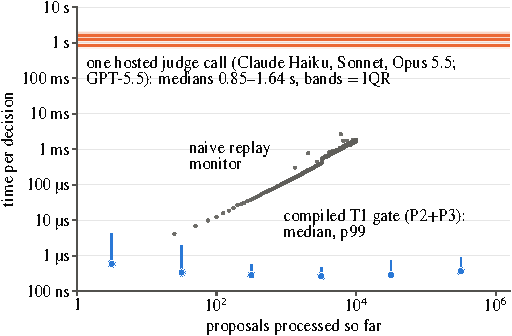
\includegraphics[width=\columnwidth]{q5_cost}
\caption{Time per decision of the compiled P2+P3 gate (blue: median and 99th
percentile in each decade of one $10^6$-proposal stream over $10^6$ recipients),
of a naive replay monitor that recomputes the policy from the committed history
for every proposal (gray; same stream, no blocks in this range), and of one hosted judge call
(orange: median and interquartile range for Claude Haiku, Sonnet, and Opus~5.5
and GPT-5.5, 24 sequential calls each, network included). Synthetic workload,
one core of an Intel i9-9820X.}
\label{fig:q5}
\end{figure}

The rule that T1 and T3 support (compile the oracle-checkable predicates, judge only
the rest) is useful only if compiled gates and their analysis are cheap. We implement
P2 and P3 as one keyed-counter gate (a hash map from active recipient--day keys to
monotone counters, plus a revocation flag) and time it in Python~3.12 on one core of an
Intel i9-9820X. Over a stream of $10^6$ proposals to $10^6$ recipients, the median
decision takes $0.26$--$0.37\,\mu$s in every decade after the first ten proposals (99th
percentile below $1\,\mu$s after the first hundred) while the state grows to
$7.7{\times}10^5$ active keys at about 110 bytes each (Figure~\ref{fig:q5}); with $10^2$
to $10^6$ recipients the median stays within $0.27$--$0.42\,\mu$s. A naive replay
monitor that recomputes the policy from the committed history for each proposal, the
literal reading of Definition~\ref{def:gate}, agrees with the gate on all
$2{\times}10^4$ proposals of two streams, one oversampling exact-cap and cap-plus-one
amounts (8,950 blocks), but its decision time grows with the history, to a median of
$0.93$\,ms at $10^3$--$10^4$ committed actions. One hosted judge call from our panel,
with the study's prompt and settings, takes a median of $0.85$\,s (Claude Haiku~5.5)
to $1.64$\,s (GPT-5.5) over 24 sequential calls, network included, about six orders
of magnitude more than the compiled check. The saturation abstraction of
Theorem~\ref{thm:frag} also supports a redundancy check for this instance: an exact
search over one saturated P2 key and the saturated session counter (exact because
deleting other keys' transfers cannot make the upper-bound limit reject;
Theorem~\ref{thm:frag} itself covers only nontriviality) finds that a per-session transfer limit $\ell$ makes P2's per-recipient cap $c$ redundant (no committed history lets
P2 block a proposal the limit allows) in each tested configuration with $\ell\le c$ and in
none with $\ell>c$, matching the analytic condition (five configurations with $c,\ell\le200$;
$21$--$508$\,ms per query). The saturated state space grows roughly
quadratically in the caps (15,251 states and $6.1{\times}10^6$ transitions at $c=100$,
$\ell=200$), so caps in fine monetary units need coarser units or a symbolic counter
encoding. On these synthetic workloads, the exact half of a guardrail is effectively
free; a gate's latency, cost, and false blocks come from the predicates it must judge.
